\documentclass[]{article}
\usepackage{lmodern}
\usepackage{amssymb,amsmath}
\usepackage{ifxetex,ifluatex}
\usepackage{fixltx2e} % provides \textsubscript
\ifnum 0\ifxetex 1\fi\ifluatex 1\fi=0 % if pdftex
  \usepackage[T1]{fontenc}
  \usepackage[utf8]{inputenc}
\else % if luatex or xelatex
  \ifxetex
    \usepackage{mathspec}
  \else
    \usepackage{fontspec}
  \fi
  \defaultfontfeatures{Ligatures=TeX,Scale=MatchLowercase}
\fi
% use upquote if available, for straight quotes in verbatim environments
\IfFileExists{upquote.sty}{\usepackage{upquote}}{}
% use microtype if available
\IfFileExists{microtype.sty}{%
\usepackage{microtype}
\UseMicrotypeSet[protrusion]{basicmath} % disable protrusion for tt fonts
}{}
\usepackage[margin=1in]{geometry}
\usepackage{hyperref}
\hypersetup{unicode=true,
            pdftitle={Homework 8},
            pdfauthor={Christophe Hunt},
            pdfborder={0 0 0},
            breaklinks=true}
\urlstyle{same}  % don't use monospace font for urls
\usepackage{color}
\usepackage{fancyvrb}
\newcommand{\VerbBar}{|}
\newcommand{\VERB}{\Verb[commandchars=\\\{\}]}
\DefineVerbatimEnvironment{Highlighting}{Verbatim}{commandchars=\\\{\}}
% Add ',fontsize=\small' for more characters per line
\usepackage{framed}
\definecolor{shadecolor}{RGB}{248,248,248}
\newenvironment{Shaded}{\begin{snugshade}}{\end{snugshade}}
\newcommand{\KeywordTok}[1]{\textcolor[rgb]{0.13,0.29,0.53}{\textbf{{#1}}}}
\newcommand{\DataTypeTok}[1]{\textcolor[rgb]{0.13,0.29,0.53}{{#1}}}
\newcommand{\DecValTok}[1]{\textcolor[rgb]{0.00,0.00,0.81}{{#1}}}
\newcommand{\BaseNTok}[1]{\textcolor[rgb]{0.00,0.00,0.81}{{#1}}}
\newcommand{\FloatTok}[1]{\textcolor[rgb]{0.00,0.00,0.81}{{#1}}}
\newcommand{\ConstantTok}[1]{\textcolor[rgb]{0.00,0.00,0.00}{{#1}}}
\newcommand{\CharTok}[1]{\textcolor[rgb]{0.31,0.60,0.02}{{#1}}}
\newcommand{\SpecialCharTok}[1]{\textcolor[rgb]{0.00,0.00,0.00}{{#1}}}
\newcommand{\StringTok}[1]{\textcolor[rgb]{0.31,0.60,0.02}{{#1}}}
\newcommand{\VerbatimStringTok}[1]{\textcolor[rgb]{0.31,0.60,0.02}{{#1}}}
\newcommand{\SpecialStringTok}[1]{\textcolor[rgb]{0.31,0.60,0.02}{{#1}}}
\newcommand{\ImportTok}[1]{{#1}}
\newcommand{\CommentTok}[1]{\textcolor[rgb]{0.56,0.35,0.01}{\textit{{#1}}}}
\newcommand{\DocumentationTok}[1]{\textcolor[rgb]{0.56,0.35,0.01}{\textbf{\textit{{#1}}}}}
\newcommand{\AnnotationTok}[1]{\textcolor[rgb]{0.56,0.35,0.01}{\textbf{\textit{{#1}}}}}
\newcommand{\CommentVarTok}[1]{\textcolor[rgb]{0.56,0.35,0.01}{\textbf{\textit{{#1}}}}}
\newcommand{\OtherTok}[1]{\textcolor[rgb]{0.56,0.35,0.01}{{#1}}}
\newcommand{\FunctionTok}[1]{\textcolor[rgb]{0.00,0.00,0.00}{{#1}}}
\newcommand{\VariableTok}[1]{\textcolor[rgb]{0.00,0.00,0.00}{{#1}}}
\newcommand{\ControlFlowTok}[1]{\textcolor[rgb]{0.13,0.29,0.53}{\textbf{{#1}}}}
\newcommand{\OperatorTok}[1]{\textcolor[rgb]{0.81,0.36,0.00}{\textbf{{#1}}}}
\newcommand{\BuiltInTok}[1]{{#1}}
\newcommand{\ExtensionTok}[1]{{#1}}
\newcommand{\PreprocessorTok}[1]{\textcolor[rgb]{0.56,0.35,0.01}{\textit{{#1}}}}
\newcommand{\AttributeTok}[1]{\textcolor[rgb]{0.77,0.63,0.00}{{#1}}}
\newcommand{\RegionMarkerTok}[1]{{#1}}
\newcommand{\InformationTok}[1]{\textcolor[rgb]{0.56,0.35,0.01}{\textbf{\textit{{#1}}}}}
\newcommand{\WarningTok}[1]{\textcolor[rgb]{0.56,0.35,0.01}{\textbf{\textit{{#1}}}}}
\newcommand{\AlertTok}[1]{\textcolor[rgb]{0.94,0.16,0.16}{{#1}}}
\newcommand{\ErrorTok}[1]{\textcolor[rgb]{0.64,0.00,0.00}{\textbf{{#1}}}}
\newcommand{\NormalTok}[1]{{#1}}
\usepackage{longtable,booktabs}
\usepackage{graphicx,grffile}
\makeatletter
\def\maxwidth{\ifdim\Gin@nat@width>\linewidth\linewidth\else\Gin@nat@width\fi}
\def\maxheight{\ifdim\Gin@nat@height>\textheight\textheight\else\Gin@nat@height\fi}
\makeatother
% Scale images if necessary, so that they will not overflow the page
% margins by default, and it is still possible to overwrite the defaults
% using explicit options in \includegraphics[width, height, ...]{}
\setkeys{Gin}{width=\maxwidth,height=\maxheight,keepaspectratio}
\IfFileExists{parskip.sty}{%
\usepackage{parskip}
}{% else
\setlength{\parindent}{0pt}
\setlength{\parskip}{6pt plus 2pt minus 1pt}
}
\setlength{\emergencystretch}{3em}  % prevent overfull lines
\providecommand{\tightlist}{%
  \setlength{\itemsep}{0pt}\setlength{\parskip}{0pt}}
\setcounter{secnumdepth}{5}
% Redefines (sub)paragraphs to behave more like sections
\ifx\paragraph\undefined\else
\let\oldparagraph\paragraph
\renewcommand{\paragraph}[1]{\oldparagraph{#1}\mbox{}}
\fi
\ifx\subparagraph\undefined\else
\let\oldsubparagraph\subparagraph
\renewcommand{\subparagraph}[1]{\oldsubparagraph{#1}\mbox{}}
\fi

%%% Use protect on footnotes to avoid problems with footnotes in titles
\let\rmarkdownfootnote\footnote%
\def\footnote{\protect\rmarkdownfootnote}

%%% Change title format to be more compact
\usepackage{titling}

% Create subtitle command for use in maketitle
\newcommand{\subtitle}[1]{
  \posttitle{
    \begin{center}\large#1\end{center}
    }
}

\setlength{\droptitle}{-2em}
  \title{Homework 8}
  \pretitle{\vspace{\droptitle}\centering\huge}
  \posttitle{\par}
  \author{Christophe Hunt}
  \preauthor{\centering\large\emph}
  \postauthor{\par}
  \predate{\centering\large\emph}
  \postdate{\par}
  \date{March 25, 2017}

\usepackage{relsize}
\usepackage{setspace}
\usepackage{amsmath,amsfonts,amsthm}
\usepackage[sfdefault]{roboto}
\usepackage[T1]{fontenc}
\usepackage{float}
\usepackage{multirow}
\usepackage{mathtools}
\usepackage{tikz}

\begin{document}
\maketitle

{
\setcounter{tocdepth}{2}
\tableofcontents
}
\section{Problem Set 1}\label{problem-set-1}

Your colleague either commutes by train or by the bus. 20 days of the
month, she takes the train and the remaining 10 days she takes the bus.
If she takes the train, she reaches work on time with a probability of
0.9. If she takes the bus, she frequently gets stuck in traffic and
reaches work on time with a probability of 0.5. Given that she was on
time today, what is the probability that she took the bus to work today?

\begin{quote}
\(P(bus|on~time) = \frac{P(on~time|bus)*P(Bus)}{P(on~time|bus)*P(Bus) + P(on~time|Train)*P(Train)}\)
\end{quote}

\begin{center}
\line(1,0){250}
\end{center}

\begin{Shaded}
\begin{Highlighting}[]
\KeywordTok{library}\NormalTok{(scales)}
\NormalTok{train <-}\StringTok{ }\DecValTok{20}\NormalTok{/}\DecValTok{30}
\NormalTok{bus <-}\StringTok{ }\DecValTok{10}\NormalTok{/}\DecValTok{30}
\NormalTok{ontime_train <-}\StringTok{ }\NormalTok{.}\DecValTok{9}
\NormalTok{ontime_bus <-}\StringTok{ }\NormalTok{.}\DecValTok{5}

\NormalTok{bus_ontime <-}\StringTok{ }\NormalTok{(ontime_bus *}\StringTok{ }\NormalTok{bus)/}\StringTok{ }\NormalTok{((ontime_bus *}\StringTok{ }\NormalTok{bus) +}\StringTok{ }\NormalTok{(ontime_train*train))}
\KeywordTok{percent}\NormalTok{(bus_ontime)}
\end{Highlighting}
\end{Shaded}

{[}1{]} ``21.7\%''

\begin{quote}
The probability that my colleague took the bus given that she is on time
is 21.7\%
\end{quote}

\newpage

\section{Problem Set 2}\label{problem-set-2}

In the Grade Network that we looked at in the notes,

\begin{figure}[htbp]
\centering
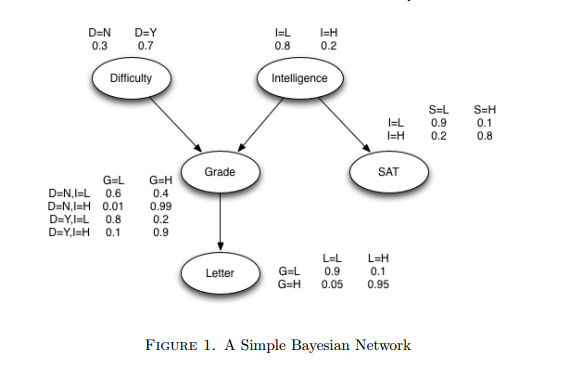
\includegraphics{https://raw.githubusercontent.com/ChristopheHunt/MSDA---Coursework/master/Data\%20605/Assignment\%208/figure1.PNG}
\caption{}
\end{figure}

\begin{Shaded}
\begin{Highlighting}[]
\KeywordTok{library}\NormalTok{(gRain)}
\CommentTok{# Build the network}
\NormalTok{n.y <-}\StringTok{ }\KeywordTok{c}\NormalTok{(}\StringTok{"no"}\NormalTok{, }\StringTok{"yes"}\NormalTok{)}
\NormalTok{l.h <-}\StringTok{ }\KeywordTok{c}\NormalTok{(}\StringTok{"low"}\NormalTok{, }\StringTok{"high"}\NormalTok{)}
\NormalTok{d <-}\StringTok{ }\KeywordTok{cptable}\NormalTok{(~difficulty, }\DataTypeTok{values =} \KeywordTok{c}\NormalTok{(}\FloatTok{0.3}\NormalTok{, }\FloatTok{0.7}\NormalTok{), }\DataTypeTok{levels =} \NormalTok{n.y)}
\NormalTok{i <-}\StringTok{ }\KeywordTok{cptable}\NormalTok{(~intelligence, }\DataTypeTok{values =} \KeywordTok{c}\NormalTok{(}\FloatTok{0.8}\NormalTok{, }\FloatTok{0.2}\NormalTok{), }\DataTypeTok{levels =} \NormalTok{l.h)}
\NormalTok{s.i <-}\StringTok{ }\KeywordTok{cptable}\NormalTok{(~sat |}\StringTok{ }\NormalTok{intelligence, }\DataTypeTok{values =} \KeywordTok{c}\NormalTok{(}\FloatTok{0.9}\NormalTok{, }\FloatTok{0.1}\NormalTok{, }\FloatTok{0.2}\NormalTok{, }\FloatTok{0.8}\NormalTok{), }\DataTypeTok{levels =} \NormalTok{l.h)}
\NormalTok{g.d.i <-}\StringTok{ }\KeywordTok{cptable}\NormalTok{(~grade |}\StringTok{ }\NormalTok{difficulty:intelligence, }\DataTypeTok{values =} \KeywordTok{c}\NormalTok{(}\FloatTok{0.6}\NormalTok{, }\FloatTok{0.4}\NormalTok{, }\FloatTok{0.8}\NormalTok{, }
    \FloatTok{0.2}\NormalTok{, }\FloatTok{0.1}\NormalTok{, }\FloatTok{0.99}\NormalTok{, }\FloatTok{0.1}\NormalTok{, }\FloatTok{0.9}\NormalTok{), }\DataTypeTok{levels =} \NormalTok{l.h)}
\NormalTok{l.g <-}\StringTok{ }\KeywordTok{cptable}\NormalTok{(~letter |}\StringTok{ }\NormalTok{grade, }\DataTypeTok{values =} \KeywordTok{c}\NormalTok{(}\FloatTok{0.9}\NormalTok{, }\FloatTok{0.1}\NormalTok{, }\FloatTok{0.5}\NormalTok{, }\FloatTok{0.95}\NormalTok{), }\DataTypeTok{levels =} \NormalTok{l.h)}
\NormalTok{p <-}\StringTok{ }\KeywordTok{compileCPT}\NormalTok{(}\KeywordTok{list}\NormalTok{(d, i, s.i, g.d.i, l.g))}
\NormalTok{pn <-}\StringTok{ }\KeywordTok{grain}\NormalTok{(p)}
\end{Highlighting}
\end{Shaded}

\newpage

\subsection{What happens to the probability of Difficulty of Course when
you present the evidence that the received recommendation letter was
good?}\label{what-happens-to-the-probability-of-difficulty-of-course-when-you-present-the-evidence-that-the-received-recommendation-letter-was-good}

\begin{Shaded}
\begin{Highlighting}[]
\NormalTok{l.g <-}\StringTok{ }\KeywordTok{setFinding}\NormalTok{(pn, }\DataTypeTok{nodes =} \KeywordTok{c}\NormalTok{(}\StringTok{"letter"}\NormalTok{), }\DataTypeTok{states =} \KeywordTok{c}\NormalTok{(}\StringTok{"high"}\NormalTok{))}
\KeywordTok{kable}\NormalTok{(}\KeywordTok{as.data.frame}\NormalTok{(}\KeywordTok{querygrain}\NormalTok{(l.g, }\DataTypeTok{nodes =} \KeywordTok{c}\NormalTok{(}\StringTok{"difficulty"}\NormalTok{), }\DataTypeTok{type =} \StringTok{"marginal"}\NormalTok{)))}
\end{Highlighting}
\end{Shaded}

\begin{longtable}[]{@{}lr@{}}
\toprule
& difficulty\tabularnewline
\midrule
\endhead
no & 0.3597003\tabularnewline
yes & 0.6402997\tabularnewline
\bottomrule
\end{longtable}

\subsection{In addition, now present the evidence that both SAT scores
were good and the letter of recommendation was good, What is the
probability of the Difficulty of Course
now?}\label{in-addition-now-present-the-evidence-that-both-sat-scores-were-good-and-the-letter-of-recommendation-was-good-what-is-the-probability-of-the-difficulty-of-course-now}

\begin{Shaded}
\begin{Highlighting}[]
\NormalTok{s.l.g <-}\StringTok{ }\KeywordTok{setFinding}\NormalTok{(}\KeywordTok{setFinding}\NormalTok{(pn, }\DataTypeTok{nodes =} \KeywordTok{c}\NormalTok{(}\StringTok{"letter"}\NormalTok{), }\DataTypeTok{states =} \KeywordTok{c}\NormalTok{(}\StringTok{"high"}\NormalTok{)), }
    \DataTypeTok{nodes =} \KeywordTok{c}\NormalTok{(}\StringTok{"sat"}\NormalTok{), }\DataTypeTok{states =} \KeywordTok{c}\NormalTok{(}\StringTok{"high"}\NormalTok{))}
\KeywordTok{kable}\NormalTok{(}\KeywordTok{as.data.frame}\NormalTok{(}\KeywordTok{querygrain}\NormalTok{(s.l.g, }\DataTypeTok{nodes =} \KeywordTok{c}\NormalTok{(}\StringTok{"difficulty"}\NormalTok{), }\DataTypeTok{type =} \StringTok{"marginal"}\NormalTok{)))}
\end{Highlighting}
\end{Shaded}

\begin{longtable}[]{@{}lr@{}}
\toprule
& difficulty\tabularnewline
\midrule
\endhead
no & 0.3174519\tabularnewline
yes & 0.6825481\tabularnewline
\bottomrule
\end{longtable}

You should use the gRain package in R to build your network and perform
these calculations.

You may need to install RBGL package from BioConductor in R to get gRain
working. See
\url{http://www.bioconductor.org/packages/release/bioc/html/RBGL.html}
for instructions on RBGL.

Please submit your assignment as an R markdown document.


\end{document}
